\documentclass[11pt,compress,t,notes=noshow, xcolor=table]{beamer}
\usepackage[]{graphicx}\usepackage[]{color}
% maxwidth is the original width if it is less than linewidth
% otherwise use linewidth (to make sure the graphics do not exceed the margin)
\makeatletter
\def\maxwidth{ %
  \ifdim\Gin@nat@width>\linewidth
    \linewidth
  \else
    \Gin@nat@width
  \fi
}
\makeatother

\definecolor{fgcolor}{rgb}{0.345, 0.345, 0.345}
\newcommand{\hlnum}[1]{\textcolor[rgb]{0.686,0.059,0.569}{#1}}%
\newcommand{\hlstr}[1]{\textcolor[rgb]{0.192,0.494,0.8}{#1}}%
\newcommand{\hlcom}[1]{\textcolor[rgb]{0.678,0.584,0.686}{\textit{#1}}}%
\newcommand{\hlopt}[1]{\textcolor[rgb]{0,0,0}{#1}}%
\newcommand{\hlstd}[1]{\textcolor[rgb]{0.345,0.345,0.345}{#1}}%
\newcommand{\hlkwa}[1]{\textcolor[rgb]{0.161,0.373,0.58}{\textbf{#1}}}%
\newcommand{\hlkwb}[1]{\textcolor[rgb]{0.69,0.353,0.396}{#1}}%
\newcommand{\hlkwc}[1]{\textcolor[rgb]{0.333,0.667,0.333}{#1}}%
\newcommand{\hlkwd}[1]{\textcolor[rgb]{0.737,0.353,0.396}{\textbf{#1}}}%
\let\hlipl\hlkwb

\usepackage{framed}
\makeatletter
\newenvironment{kframe}{%
 \def\at@end@of@kframe{}%
 \ifinner\ifhmode%
  \def\at@end@of@kframe{\end{minipage}}%
  \begin{minipage}{\columnwidth}%
 \fi\fi%
 \def\FrameCommand##1{\hskip\@totalleftmargin \hskip-\fboxsep
 \colorbox{shadecolor}{##1}\hskip-\fboxsep
     % There is no \\@totalrightmargin, so:
     \hskip-\linewidth \hskip-\@totalleftmargin \hskip\columnwidth}%
 \MakeFramed {\advance\hsize-\width
   \@totalleftmargin\z@ \linewidth\hsize
   \@setminipage}}%
 {\par\unskip\endMakeFramed%
 \at@end@of@kframe}
\makeatother

\definecolor{shadecolor}{rgb}{.97, .97, .97}
\definecolor{messagecolor}{rgb}{0, 0, 0}
\definecolor{warningcolor}{rgb}{1, 0, 1}
\definecolor{errorcolor}{rgb}{1, 0, 0}
\newenvironment{knitrout}{}{} % an empty environment to be redefined in TeX

\usepackage{alltt}
\newcommand{\SweaveOpts}[1]{}  % do not interfere with LaTeX
\newcommand{\SweaveInput}[1]{} % because they are not real TeX commands
\newcommand{\Sexpr}[1]{}       % will only be parsed by R



\usepackage[english]{babel}
\usepackage[utf8]{inputenc}

\usepackage{dsfont}
\usepackage{verbatim}
\usepackage{amsmath}
\usepackage{amsfonts}
\usepackage{bm}
\usepackage{csquotes}
\usepackage{multirow}
\usepackage{longtable}
\usepackage{booktabs}
\usepackage{enumerate}
\usepackage[absolute,overlay]{textpos}
\usepackage{psfrag}
\usepackage{algorithm}
\usepackage{algpseudocode}
\usepackage{eqnarray}
\usepackage{arydshln}
\usepackage{tabularx}
\usepackage{placeins}
\usepackage{tikz}
\usepackage{setspace}
\usepackage{colortbl}
\usepackage{mathtools}
\usepackage{wrapfig}
\usepackage{bm}
\usetikzlibrary{shapes,arrows,automata,positioning,calc,chains,trees, shadows}
\tikzset{
  %Define standard arrow tip
  >=stealth',
  %Define style for boxes
  punkt/.style={
    rectangle,
    rounded corners,
    draw=black, very thick,
    text width=6.5em,
    minimum height=2em,
    text centered},
  % Define arrow style
  pil/.style={
    ->,
    thick,
    shorten <=2pt,
    shorten >=2pt,}
}
\usepackage{subfig}


% Defines macros and environments
\input{../../style/common.tex}
% \input{common.tex}

%\usetheme{lmu-lecture}
\newcommand{\titlefigure}{figure_man/cart-labelling_of_tree-new.pdf}
\newcommand{\learninggoals}{
\item Understand the basic structure of a tree model
\item Understand that the basic idea of a tree model is the same for classification and regression 
\item Know how the label of a new observation is predicted via CART
\item Know hypothesis space of CART}
\usepackage{../../style/lmu-lecture}

\let\code=\texttt
\let\proglang=\textsf

\setkeys{Gin}{width=0.9\textwidth}

\title{Introduction to Machine Learning}
% \author{Bernd Bischl, Christoph Molnar, Daniel Schalk, Fabian Scheipl}
\institute{\href{https://compstat-lmu.github.io/lecture_i2ml/}{compstat-lmu.github.io/lecture\_i2ml}}
\date{}

\setbeamertemplate{frametitle}{\expandafter\uppercase\expandafter\insertframetitle}



\begin{document}
% Set style/preamble.Rnw as parent.


% Defines macros and environments
\input{../../latex-math/basic-math.tex}
\input{../../latex-math/basic-ml.tex}


%! includes: basics-riskminimization, regression-losses, classification-basicdefs

% Load all R packages and set up knitr

% This file loads R packages, configures knitr options and sets preamble.Rnw as parent file
% IF YOU MODIFY THIS, PLZ ALSO MODIFY setup.Rmd ACCORDINGLY...









\lecturechapter{Classification and Regression Trees (CART): Basics}
\lecture{Introduction to Machine Learning}
\sloppy



\begin{vbframe}{Tree Model and Prediction}
    \begin{figure}
    \centering
      % FIGURE SOURCE: No source
      %\includegraphics[height = 4.5cm]{figure_man/labelling_of_tree.png}
      %figure/cart_intro_5_with_tree.pdf
      % https://docs.google.com/drawings/d/1WZrSJ5QldA7VYjE5U9gGPCiTFyhWYHJI-37k7G2jXI8/edit?usp=sharing
      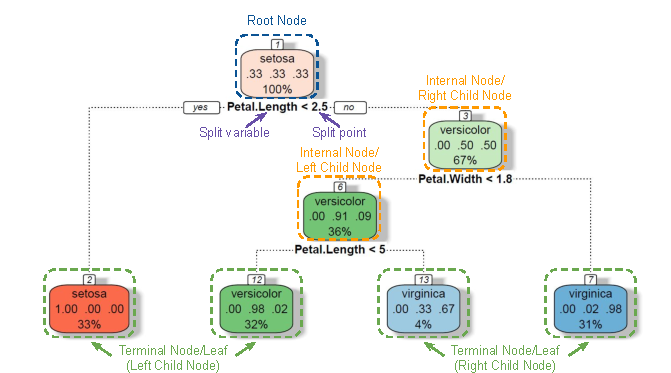
\includegraphics[height = 5cm,keepaspectratio]{figure_man/cart-labelling_of_tree-new.pdf}
    \end{figure}
  \begin{itemize}
    \item Classification and Regression Trees, introduced by Breiman
    \item Binary splits are constructed top-down
    \item Constant prediction in each terminal node (leaf): either a numerical value,
  a class label, or a probability vector over class labels.
  \end{itemize}
\end{vbframe}

\begin{vbframe}{Tree Model and Prediction}
  \begin{itemize}
    \item For predictions, observations are passed down the tree, according to the splitting rules
      in each node
    \item An observation will end up in exactly one leaf node
    \item All observations in a leaf node are assigned the same prediction for the target
  \end{itemize}
    \begin{figure}
    \centering
      % FIGURE SOURCE: No source
      %\includegraphics[height = 4.5cm]{figure_man/labelling_of_tree.png}
      
      %figure/cart_intro_5_with_tree.pdf
      % https://docs.google.com/drawings/d/1OdrK3Vb-IAObjMV98730c0wZ5ohnQ7ZbvGtQRZHPsTE/edit?usp=sharing
      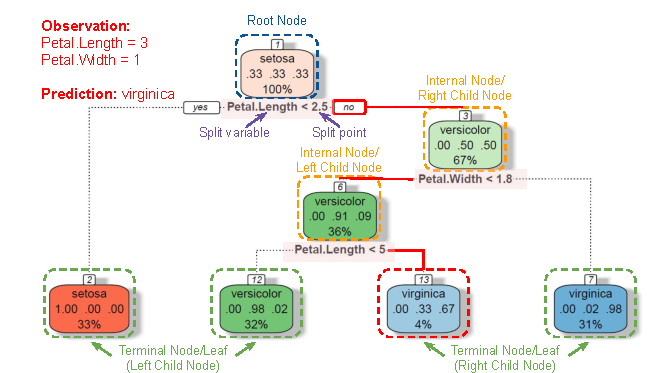
\includegraphics[height = 5cm,keepaspectratio]{figure_man/cart-labelling_of_tree-new-example.pdf}
    \end{figure}
\end{vbframe}

\begin{vbframe}{Tree Model and Prediction}
  \begin{itemize}
    \item For predictions, observations are passed down the tree, according to the splitting rules
      in each node
    \item An observation will end up in exactly one leaf node
    \item All observations in a leaf node are assigned the same prediction for the target
  \end{itemize}
    \begin{figure}
    \centering
      % FIGURE SOURCE: No source
      \includegraphics[height = 4.5cm]{figure_man/CART_reg_example.pdf}
    \end{figure}
\end{vbframe}


\begin{vbframe}{Tree as an additive model}
Each point in $\Xspace$ is assigned to exactly one leaf, and each leaf has a set of input points leading to it through axis-parallel splits.\\
Hence, trees divide the feature space $\Xspace$ into \textbf{rectangular regions}: 
  \begin{align*}
    \fx = \sum_{m=1}^M c_m \I(\xv \in Q_m),
  \end{align*}
  where a tree with $M$ leaf nodes defines $M$ \enquote{rectangles} $Q_m$.\\
  $c_m$ is the predicted numerical response, class label or class
  distribution in the respective leaf node.

\centering 
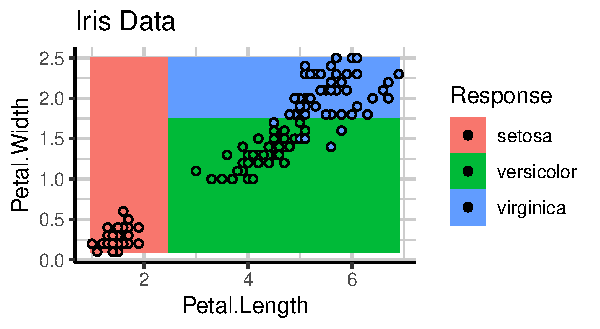
\includegraphics[width=0.45\textwidth, page = 1]{figure/cart_intro_1_with_tree}
\includegraphics[width=0.45\textwidth, page = 2]{figure/cart_intro_1_with_tree} 


\end{vbframe}

\begin{frame}[fragile]{Trees}

The hypothesis space of a CART is the set of all step functions over rectangular partitions of $\Xspace$:
\begin{align*}
    \fx = \sum_{m=1}^M c_m \I(\xv \in Q_m)
\end{align*}

\begin{columns}
\begin{column}{0.5\textwidth}
Classification:
\lz
\begin{knitrout}\scriptsize
\definecolor{shadecolor}{rgb}{0.969, 0.969, 0.969}\color{fgcolor}

{\centering \includegraphics[width=0.95\textwidth]{figure/cart_intro_2} 

}



\end{knitrout}
 
\end{column}
\begin{column}{0.5\textwidth}
Regression:

\includegraphics[height = 0.4\textheight]{figure_man/CART_reg_example.pdf}

\end{column}
\end{columns}
\end{frame}








% % BB: as we are not really talking too much about impurity anymore, I took this out
% % <<splitcriteria-plot, results='hide', fig.height=5>>=
% % Colors = pal_3
% % par(mar = c(5.1, 4.1, 0.1, 0.1))
% % p = seq(1e-6, 1-1e-6, length.out = 200)
% % entropy = function(p) (p * log(p) + (1 - p) * log(1 - p))/(2 * log(0.5))
% % gini = function(p) 2 * p * (1 - p)
% % missclassification = function(p) (1 - max(p, 1 - p))
% % plot(p, entropy(p), type = "l", col = Colors[1], lwd = 1.5, ylab = "",
% %   ylim = c(0, 0.6), xlab = expression(hat(pi)[Nk]))
% % lines(p, gini(p), col = Colors[2], lwd = 1.5)
% % lines(p, sapply(p, missclassification), col = Colors[3], lwd = 1.5)
% % legend("topright", c("Gini Index", "Entropy", "Misclassification Error"),
% %        col = Colors[1:3], lty = 1)
% % @


\endlecture
\end{document}
